
\newcommand{\khungmuiten}[2][\mycolor]{
	\begin{tikzpicture}[declare function ={r=8cm;d=.04*r;}]
		\node(char)[font=\bfseries\sffamily,inner sep =2pt]{\tikz{
				\path (0,0)--(r,0) node[pos=0.5,midway]{#2};
		}};
		\path (char.north west) coordinate (A)
		(char.south west) coordinate (D)
		(char.north east) coordinate (B)
		([yshift=d]char.north east) coordinate (Bt)
		([xshift=2*d]char.east) coordinate (BtC)
		(char.south east) coordinate (C)
		([yshift=-d]char.south east) coordinate (Ct)
		;
		\filldraw [fill=#1!20,draw=#1!50!black,inner sep =1pt](A)--(B)--(Bt)--(BtC)--(Ct)--(C)--(D)--cycle;
		\node(char)[font=\bfseries\sffamily,inner sep =2pt]{\tikz{
				\path (0,0)--(4,0) node[pos=0.5,midway]{#2};
		}};
\end{tikzpicture}}
\newtcolorbox{body}{%
	before skip=1cm,
	colback=\mycolor!20,
	enhanced jigsaw,opacityback=0,opacitybacktitle=0,
	opacityback=0,
	colframe=\mycolor
}
\renewcommand*\printatom[1]{\ensuremath{\mathbf{#1}}}
\newcommand*\mynode[1]{%
	\begin{tikzpicture}[remember picture]
		\node [%
		rectangle,
		rounded corners =3pt,
		minimum height =1cm,
		minimum width = .65cm,
		anchor=center, 
		fill = \maunhan!20,
		draw=\maunhan
		]
		{\printatom{#1}};
	\end{tikzpicture}
}
\renewcommand{\hinhphai}[2]{%
	\tcbsidebyside[
	sidebyside adapt=right,
	blanker,sidebyside gap=3mm,
	sidebyside align=top seam,
	]{%
		#1
	}{%
		#2
	}
}
\section{Hợp chất hữu cơ và hóa học hữu cơ}
\begin{tcolorbox}[colframe=\mycolor!50!black,colback=\mycolor!20,arc is angular,arc=0pt]
	\begin{center}
		{\bf\Large\color{\mycolor!50!black}\MakeUppercase{Nhận biết các nhóm chức trong phổ hồng ngoại}}
	\end{center}
\end{tcolorbox}
\paragraph{Đặc điểm nhận biết nhóm carbonyl}

\hinhphai{\begin{itemize}
		\item Tín hiệu mạnh 
		\item Có mặt trong nhiều nhóm chức
		\item Có thể phân biệt dễ dàng ở số sóng \indam{1700 - 1800 $cm^{-1}$}
\end{itemize}}{
\begin{tikzpicture}[declare function={d=1.35pt;},node distance=.8cm,scale=1.25]
	\node[font=\Large\bf](C) {C};
	\node[right= of C,font=\Large\bf](R) {};
	\node[above=.55cm of C,font=\Large\bf](O) {O};
	\node[left=.65cm of C,font=\Large\bf](CH3) {\vphantom{CH3}};
	\filldraw[fill=\maunhan!20,rounded corners=3pt,opacity=.5] (O.north west) rectangle (C.south east);
	\node[font=\Large\bf](C) {C};
	\node[above=.55cm of C,font=\Large\bf](O) {O};
	\draw[thick] ([xshift=-d]C.north)--([xshift=-d]O.south);
	\draw[thick] ([xshift=d]C.north)--([xshift=d]O.south);
	\draw[thick] (CH3)--([xshift=2pt]C.west) ([xshift=-2pt]C.east)--(R) ;
	\node[below=3pt of C,font=\bf](Peak){Vân hấp thụ : 1700 -- 1800 $\mathbf{cm}^{\textbf{-1}}$};
\end{tikzpicture}}
\paragraph{Vân hấp thụ của nhóm carbonyl (C=O) trong một số hợp chất}

\begin{itemize}
	\item Khi nhóm C=O liên kết với các nguyên tố \indam{độ âm điện càng lớn} vân hấp thụ của nhóm C=O dịch chuyển về \indam{số sóng lớn hơn} (xem hình \ref{fig:carbonyl})
	\item Liên kết \indam{càng phân cực} thì vân hấp thụ dịch chuyển về \indam{số sóng ngắn hơn} (xem hình \ref{fig:moment})
	\item Độ bền \indam{liên kết càng tăng} thì vân hấp thụ chuyển dịch về \indam{số sóng lớn hơn} (xem hình \ref{fig:bondstrength} và \ref{fig:bondstrength1} )
	\item Khi nhóm chức \indam{có tạo liên kết hidro }vân hấp thụ sẽ dịch chuyển về \indam{số sóng thấp hơn} so với nhóm chức tự do (Xem hình \ref{fig:Hbond}).
\end{itemize}
%%%===============================%%%%%
\tikzstyle{colornode} = [font=\color{\maunhan}\bfseries\sffamily]
\begin{body}
\begin{tikzpicture}[declare function={d=1.35pt;r=4.0cm;},node distance=0.8cm,inner sep=2pt]
	\tikzset{pics/.cd,
		carbonyl/.style args={#1/#2}{code={
				\node[font=\Large\bf](C) {C};
				\node[right= of C,font=\Large\bf](R) {#1};
				\node[above=.55cm of C,font=\Large\bf](O) {O};
				\node[left=.65cm of C,font=\Large\bf](CH3) {\vphantom{CH3}};
				\filldraw[fill=\maunhan!20,rounded corners=3pt,opacity=.5] (O.north west) rectangle (C.south east);
				\node[font=\Large\bf](C) {C};
				\node[above=.55cm of C,font=\Large\bf](O) {O};
				\draw[thick] ([xshift=-d]C.north)--([xshift=-d]O.south);
				\draw[thick] ([xshift=d]C.north)--([xshift=d]O.south);
				\draw[thick] (CH3)--([xshift=2pt]C.west) ([xshift=-2pt]C.east)--(R) ;
				\node[below=3pt of C,colornode](Peak){#2 $\mathbf{cm}^{\textbf{-1}}$};	
			}
		}
	}
	\pic[local bounding box =Ketones] at (0,0){carbonyl={R}/{1710}};
	\pic[local bounding box =Aldehydes] at (r,0){carbonyl={H}/{1720}};
	\pic[local bounding box =Acids] at (2*r,0){carbonyl={OH}/{1730}};
	\pic[local bounding box =Ester] at (3*r,0){carbonyl={OR}/{1750}};
	\pic[local bounding box =Amid] at (0,-r){carbonyl={$NH_2$}/{1770}};
	\pic[local bounding box =Acid halides] at (r,-r){carbonyl={X}/{1800}};
	\pic[local bounding box =Anhydrics1] at (2*r,-r){carbonyl={O}/{1810}};
	\pic[local bounding box =Anhydrics] at (2.655*r,-r){carbonyl={}/{1760}};
	\foreach \x/\y in {Ketones/5,Aldehydes/5,Acids/14,Ester/12,Anhydrics/38,Amid/17,Acid halides/5}{\node [above=4pt of \x,xshift=-\y pt]{\x};}
\end{tikzpicture}
\captionof{figure}{Vân hấp thụ của nhóm carbonyl trong một số hợp chất \label{fig:carbonyl}}
\end{body}
%%%===========================================%%%
\begin{body}
	\begin{center}
		\begin{tikzpicture}[declare function={d=4cm;},node distance=0.8cm,scale=0.4]
		\node (CCl){\Large\chemfig[bond offset=2pt,atom sep=1.5cm,bond style={thick}]{C-Cl}};
		\node (CH)[right = d of CCl] {\Large\chemfig[bond offset=2pt,atom sep=1.5cm,bond style={ thick}]{C-H}};
		\node [below= 3pt of CCl,colornode] {750 $\textsf{cm}^{\textsf{-1}}$ };
		\node [above= 3pt of CCl,colornode] {Momen lưỡng cực lớn };
		\node [below= 3pt of CH,colornode] {2960 $\textsf{cm}^{\textsf{-1}}$ };
		\node [above= 3pt of CH,colornode] {Momen lưỡng cực nhỏ };
		\end{tikzpicture}
		\captionof{figure}{Vân hấp thụ của các liên kết có moment lưỡng cực khác nhau \label{fig:moment}}
	\end{center}
\end{body}

\begin{body}
	\begin{center}
		\begin{tikzpicture}[declare function={d=3cm;},node distance=0.8cm,scale=0.4]
			\node (C){\Large\chemfig[bond offset=2pt,atom sep=1.5cm,bond style={thick}]{C-C}};
			\node (CC)[right = d of C] {\Large\chemfig[bond offset=2pt,atom sep=1.5cm,bond style={ thick}]{C=C}};
			\node (CCC) [right = d of CC,font=\sffamily\bfseries] {\Large\chemfig[bond offset=2pt,atom sep=1.5cm,bond style={thick}]{C~C}};
			\node [below= 3pt of C,colornode] {1200 $\textsf{cm}^{\textsf{-1}}$ };
			\node [below= 3pt of CC,colornode] {1650 $\textsf{cm}^{\textsf{-1}}$ };
			\node [below= 3pt of CCC,colornode] {2150 $\textsf{cm}^{\textsf{-1}}$ };
		\end{tikzpicture}
		\khungmuiten[cyan]{Số sóng hấp thụ tăng theo độ bền liên kết}
		\captionof{figure}{Vân hấp thụ các liên kết có độ bền khác nhau \label{fig:bondstrength}}
	\end{center}
\end{body}

\begin{body}
	\begin{center}
		\begin{tikzpicture}[declare function={d=3cm;},node distance=0.8cm,scale=0.4]
			\node (CH){\Large\chemfig[bond offset=2pt,atom sep=1.5cm,bond style={thick}]{C-H}};
			\node (NH)[right = d of CH] {\Large\chemfig[bond offset=2pt,atom sep=1.5cm,bond style={ thick}]{N-H}};
			\node (OH) [right = d of NH,font=\sffamily\bfseries] {\Large\chemfig[bond offset=2pt,atom sep=1.5cm,bond style={thick}]{O-H}};
			\node [below= 3pt of CH,colornode] {2960 $\textsf{cm}^{\textsf{-1}}$ };
			\node [below= 3pt of NH,colornode] {3300 $\textsf{cm}^{\textsf{-1}}$ };
			\node [below= 3pt of OH,colornode] {3600 $\textsf{cm}^{\textsf{-1}}$ };
		\end{tikzpicture}
		\khungmuiten[cyan]{Số sóng hấp thụ tăng theo độ bền liên kết}
		\captionof{figure}{Vân hấp thụ các liên kết có độ bền khác nhau \label{fig:bondstrength1}}
	\end{center}
\end{body}

\begin{body}
	\begin{center}
		\begin{tikzpicture}
			\node (LKH){\large \chemfig[atom style={\mycolor},bond style={\mycolor}]{\charge{-90:2pt[red,anchor=90]=$\delta^{-} $}{O}(-[:120]R)-\charge{60:2pt[red,anchor=-90]=$\delta^{+} $}{H}-[,1.25,,,hidrobond={+}/{2.5em}/{red}]\charge{-90:2pt[red,anchor=90]=$\delta^{-} $}{O}(-[:120]R)-\charge{60:2pt[red,anchor=-90]=$\delta^{+} $}{H}} };
			\node [below= 0.75cm of LKH,colornode]{3200 -- 3400 $\textsf{cm}^{\textsf{-1}}$ };
			\node(KLKH)[left = 2.5cm of LKH]{\large \chemfig[atom style={\mycolor},bond style={\mycolor}]{\charge{-90:2pt[red,anchor=90]=$\delta^{-} $}{O}(-[:120]R)-\charge{60:2pt[red,anchor=-90]=$\delta^{+} $}{H}}};
			\node [below= 0.75cm of KLKH,colornode]{3600 $\textsf{cm}^{\textsf{-1}}$ };
		\end{tikzpicture}\vspace*{1.25cm}
		\captionof{figure}{Vân hấp thụ của nhóm OH tự do và OH tạo liên kết H \label{fig:Hbond}}
	\end{center}
\end{body}
\paragraph{Phân biệt vân hấp thụ một số nhóm chức}

%%%==============Bảng so sánh phổ IR của andehit và xeton===================%%%
\begin{table}[thp]
	\caption{\bfseries {So sánh vân hấp thụ của andehit và xeton}}
	\begin{tikzpicture}[declare function={d=1.35pt;r=4.0cm;},node distance=0.8cm,inner sep=2pt]
		\tikzset{pics/.cd,
		carbonyl/.style args={#1}{code={
				\node[font=\Large\bf](C) {C};
				\node[right= of C,font=\Large\bf](R) {#1};
				\node[above=.55cm of C,font=\Large\bf](O) {O};
				\node[left=.65cm of C,font=\Large\bf](CH3) {\vphantom{CH3}};
				\filldraw[fill=\maunhan!20,rounded corners=3pt,opacity=.5] (O.north west) rectangle (C.south east);
				\node[font=\Large\bf](C) {C};
				\node[above=.55cm of C,font=\Large\bf](O) {O};
				\draw[thick] ([xshift=-d]C.north)--([xshift=-d]O.south);
				\draw[thick] ([xshift=d]C.north)--([xshift=d]O.south);
				\draw[thick] (CH3)--([xshift=2pt]C.west) ([xshift=-2pt]C.east)--(R) ;
			}
		},
	}
	\tikzstyle{fontnode} = [font=\color{\maunhan}\bfseries\sffamily,]
	\tikzstyle{mynode} =[
%	draw=\mycolor!90!black,
	font=\bfseries,
	line width =.8pt,
	anchor=base ,
	align =center,
	]
	%%%==================%%%
	\tikzstyle{mymatrix} = [
	matrix of nodes,
	nodes in empty cells,
	nodes={mynode},
	column sep=-\pgflinewidth,
	row sep = -\pgflinewidth,
	minimum width = .45\linewidth,
	minimum height = 3cm,
	%%%==================%%%
	row 1/.style={
		minimum height = 1.2cm,
		nodes={
			fill=\mycolor!25,
			font=\color{\maunhan}\bfseries\fontfamily{qag}\selectfont,
		},
	},
		row 2/.style={
		minimum height = 2.2cm,
	},
		row 3/.style={
		minimum height = 1.2cm,
	},
		row 4/.style={
		minimum height = 0.90cm,
	},
	row 5/.style={
		minimum height = 3.90cm,
	},
	]
	%%%=======================================================%%%
	$\matrix(m) [mymatrix]{
		Aldehitdes & Ketonnes\\
		           &         \\
			       &        \\
		 		   &        \\
		 		   &        \\
	};$
\pic[local bounding box =Aldehydes] at ([yshift=-.5cm]m-2-1){carbonyl={H}};
\pic[local bounding box =Xeton] at ([yshift=-.5cm]m-2-2){carbonyl={R}};
\node[fontnode] at (m-3-1) {C=O: 1720 $\textbf{cm}^{\textbf{-1}}$};
\node[fontnode] at (m-3-2) {C=O: 1710 - 1720 $\textbf{cm}^{\textbf{-1}}$};
\node[fontnode] at (m-4-1) {C=H: 2960 $\textbf{cm}^{\textbf{-1}}$};
\node[fontnode] at (m-4-2) {Không có};
\draw[\maunhan,ultra thick,line join =round] (m-1-1.south west)--(m-1-2.south east);
\node (andehit) at (m-5-1) {
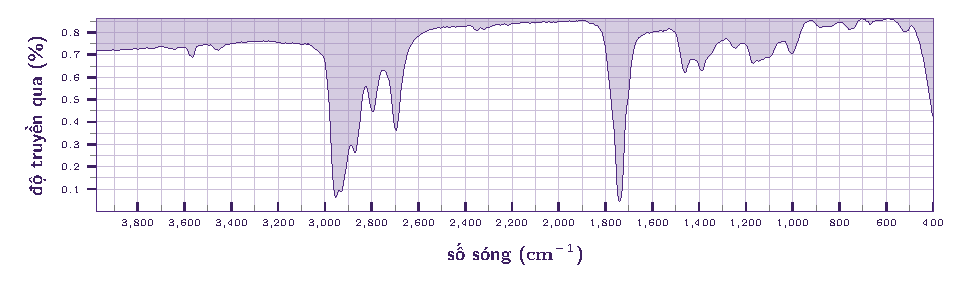
\includegraphics[width=8cm]{Images/anhphoIR/pentanal.pdf}
};
\node (xeton) at (m-5-2) {
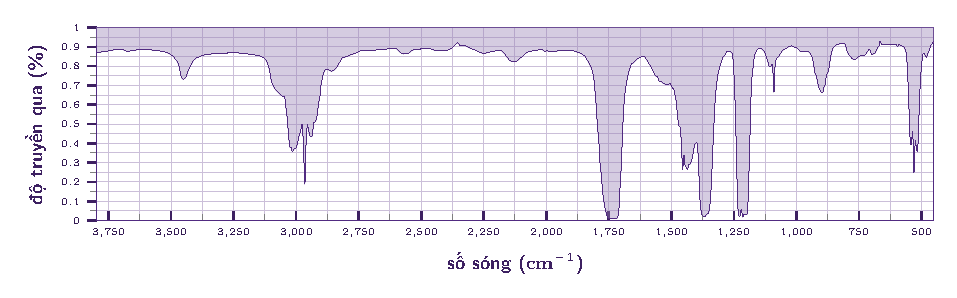
\includegraphics[width=8cm]{Images/anhphoIR/acetone.pdf}
};
\draw[\maunhan,ultra thick,rounded corners =3pt] (m-1-1.north west) rectangle (m-5-2.south east);

\draw [\maunhan,line width=1pt] ([shift={(1.15cm,0.75cm)}]andehit.south) circle (7pt);
\node(CO1)[font=\sffamily\tiny,\maunhan,text width =2cm,align=center] at ([shift={(0.15cm,1.15cm)}]andehit.south) {Vân hấp thụ nhóm C=O};
\draw [\maunhan,line width=1pt] ([shift={(1.08cm,0.75cm)}]xeton.south) circle (7pt);
 \node(CO)[font=\sffamily\tiny,\maunhan,text width =2cm,align=center] at ([shift={(0.2cm,1.15cm)}]xeton.south) {Vân hấp thụ nhóm C=O};
 \draw[\mauphu,line width=1pt] ([shift={(-.84cm,-.9cm)}]andehit.north) circle (5pt);
 \node[\mauphu,font=\sffamily\tiny] (CH) at ([shift={(0.44cm,-.9cm)}]andehit.north){Vân hấp thụ nhóm C-H};
 \path ([shift={(-.44cm,-.9cm)}]xeton.north) node[font=\sffamily\tiny,text width =3cm,align =center,\mauphu] {Không có vân hấp thụ nhóm C-H};
\end{tikzpicture}
\end{table}

%%%==============Bảng so sánh phổ IR của Axit và Ancohol===================%%%
\begin{table}[thp]
	\caption{\bfseries{So sánh vân hấp thụ của Axit và alcohol}}
	\begin{tikzpicture}[declare function={d=1.35pt;r=4.0cm;},node distance=0.8cm,inner sep=2pt]
	\tikzset{pics/.cd,
		carbonyl/.style args={#1}{code={
				\node[font=\Large\bf](C) {C};
				\node[right= of C,font=\Large\bf](R) {#1};
				\node[above=.55cm of C,font=\Large\bf](O) {O};
				\node[left=.65cm of C,font=\Large\bf](CH3) {\vphantom{CH3}};
				\filldraw[fill=\maunhan!20,rounded corners=3pt,opacity=.5] (O.north west) rectangle (C.south east);
				\node[font=\Large\bf](C) {C};
				\node[above=.55cm of C,font=\Large\bf](O) {O};
				\draw[thick] ([xshift=-d]C.north)--([xshift=-d]O.south);
				\draw[thick] ([xshift=d]C.north)--([xshift=d]O.south);
				\draw[thick] (CH3)--([xshift=2pt]C.west) ([xshift=-2pt]C.east)--(R) ;
			}
		},
		ch/.style args={#1}{code={
				\node[font=\Large\bf](C) {C};
				\node[right= of C,font=\Large\bf](R) {#1};
				\node[above=.55cm of C,font=\Large\bf](O) {H};
				\node[left=.65cm of C,font=\Large\bf](CH3) {\vphantom{CH3}};
				\filldraw[fill=\maunhan!20,rounded corners=3pt,opacity=.5] (O.north west) rectangle (C.south east);
				\node[font=\Large\bf](C) {C};
				\node[above=.55cm of C,font=\Large\bf](O) {H};
				\draw[thick]  (C.north)--(O.south);
				\draw[thick] (CH3)--([xshift=2pt]C.west) ([xshift=-2pt]C.east)--(R) ;
				\draw[thick] ([yshift=1pt]C.south)--++(-90:.35cm) ;
			}
		},
	}
	\tikzstyle{fontnode} = [font=\color{\maunhan}\bfseries\sffamily,]
	\tikzstyle{mynode} =[
%	draw=\mycolor!90!black,
	font=\bfseries,
	line width =.8pt,
	anchor=center,
	align =center,
	]
	%%%==================%%%
	\tikzstyle{mymatrix} = [
	matrix of nodes,
	nodes in empty cells,
	nodes={mynode},
	column sep=-\pgflinewidth,
	row sep = -\pgflinewidth,
	minimum width = 0.45\linewidth,
	minimum height = .65cm,
	%%%==================%%%
	row 1/.style={
		minimum height = 1.2cm,
		nodes={
			fill=\mycolor!25,
			font=\Large\color{\maunhan}\bfseries\fontfamily{qag}\selectfont,
		},
	},
	row 2/.style={
		minimum height = 2.4cm,
	},
	row 6/.style={
		minimum height = 4.6cm,
	},
	]
	%%%=======================================================%%%
	$\matrix(m) [mymatrix]{
		Axids & alcohol\\
		 	  & \\
		 	  & \\
		 	  & \\
		 	  & \\
		 	  & \\
	};$
	\pic[local bounding box =Aldehydes] at ([yshift=-.5cm]m-2-1){carbonyl={OH}};
	\pic[local bounding box =Aldehydes] at ([yshift=-.5cm]m-2-2){ch={OH}};
	\node[fontnode] at (m-3-1) {O-H: 3600 $\textbf{cm}^{\textbf{-1}}$};
	\node[fontnode] at (m-3-2) {O-H: 3600 $\textbf{cm}^{\textbf{-1}}$};
	\node[fontnode] at (m-4-1) {C-O: 1200 $\textbf{cm}^{\textbf{-1}}$};
	\node[fontnode] at (m-4-2) {C-O: 1100 $\textbf{cm}^{\textbf{-1}}$};
	\node[fontnode] at (m-5-1) {C=O: 1730 $\textbf{cm}^{\textbf{-1}}$};
	\node[fontnode] at (m-5-2) {Không có};
	\draw [\mycolor,ultra thick,rounded corners =3pt] (m-1-1.south west)--(m-1-2.south east);
	\node(Axids) at (m-6-1){
		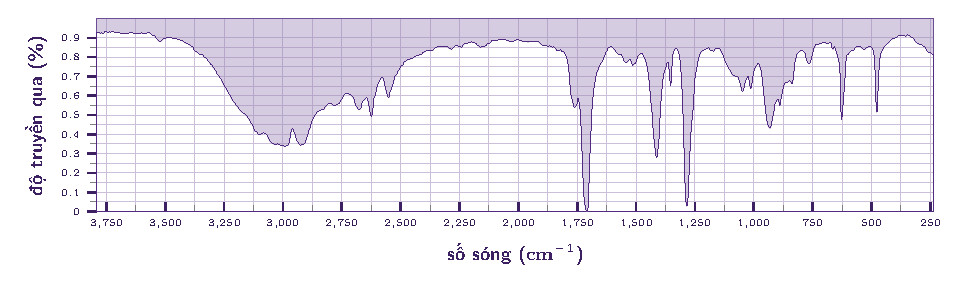
\includegraphics[width=8cm]{
		 Images/anhphoIR/Acidaxetic.pdf}
		};
	\node(Ancohol) at (m-6-2){
		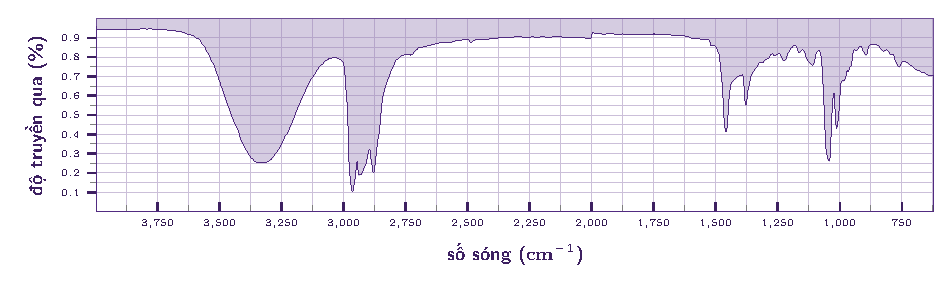
\includegraphics[width=8cm]{
		Images/anhphoIR/2methylbutan1ol.pdf}
		};
	\draw [\mycolor,ultra thick,rounded corners =3pt] (m-1-1.north west) rectangle (m-6-2.south east);
	\draw[\maunhan] ([xshift=-1.7cm]Axids) circle (8pt) node[below,font=\tiny,yshift=-6pt]{Vân hấp thụ của nhóm O-H};
	\draw[\mauphu,] ([shift={(.9cm,.8cm)}]Axids.south) circle (6pt)node[below,font=\sffamily\tiny,yshift=21pt,text width =2cm,align=center,xshift=-22pt]{Vân hấp thụ của nhóm C=O};
	\draw[\maunhan,] ([xshift=-1.8cm]Ancohol) circle (8pt)node[below,font=\tiny,yshift=-7pt,text width =2cm,align =center]{Vân hấp thụ của nhóm O-H};
	\draw[\maudam,] ([shift={(3.0cm,1.3cm)}]Ancohol.south) circle (6pt)node[below,font=\tiny,yshift=-7pt,text width =2cm,align =center]{Vân hấp thụ của nhóm C-O};
	\draw[\maudam,text width =2cm,align =center] ([shift={(1.7cm,.8cm)}]Axids.south) circle (6pt)node[below,font=\sffamily\tiny,yshift=-4pt]{Vân hấp thụ của nhóm C-O};
	 
\end{tikzpicture}
\end{table}
%%%===============Môi Trường Matrix=================%%%	







